\documentclass[a4paper]{article}

%\setlength{\parskip}{0.5\baselineskip}

\usepackage{geometry}
\geometry{left = 2.54 cm, right = 2.54 cm, top = 2.54 cm, bottom = 2.54 cm}

\usepackage{setspace}
\renewcommand{\baselinestretch}{1.0}
\usepackage{indentfirst}
\setlength{\parindent}{2em}

%\usepackage{fontspec}
%\setmainfont{Times New Roman}

\usepackage[]{cprotect}

\usepackage{hyperref}
\hypersetup{
  colorlinks=true,
  linkcolor=blue,
  filecolor=magenta,
  urlcolor=cyan,
}

\usepackage{ulem}
\usepackage{graphicx}
%\usepackage{wrapfig}
\usepackage{enumitem}
\usepackage{xcolor}
\usepackage{subcaption}
\usepackage{float}
\usepackage{amsmath, amssymb, amsthm}
\usepackage{booktabs}

\usepackage{listings} % Required for insertion of code

\lstdefinestyle{lzx}{
    % basicstyle = \small\ttfamily\fontfamily{cmr}\selectfont,
    basicstyle = \ttfamily \footnotesize,
    keywordstyle = \color{purple}\bfseries,
    % commentstyle = \color{green}\itshape,
    commentstyle = \color[RGB]{116, 153, 62}\ttfamily,
    stringstyle = \ttfamily,
    %
    tabsize = 2,
    showspaces = false,
    numberstyle = \ttfamily\color[RGB]{0,96,96},
    showstringspaces = false,
    captionpos = t,
    %
    showlines = true,
    emptylines = *2, % 2 for python, 1 for other language
    numbers = left,
    xleftmargin = 5mm,
    numbersep = 5pt,
    linewidth = \linewidth,
    % backgroundcolor=\color{red},
    frame = single,
    frameround = tttt,
    framexleftmargin = 7mm,
    %
    breaklines = true,
    postbreak = \mbox{\textcolor{red}{\( \hookrightarrow \)}\space},
}

\lstset{
    style = lzx, %
}

%\pagestyle{empty} % Not showing page number

\begin{document}
\renewcommand{\thesection}{\Roman{section}}
\renewcommand{\thesubsection}{\Alph{subsection}}
\renewcommand{\thesubsubsection}{\thesubsection.\arabic{subsubsection}}
\renewcommand{\d}{\: \mathrm{d}}
\newcommand{\e}{\mathrm{e}}

\begin{center}
  \textbf{\Large VE373 Recitation Class}\\[1em]
  \textbf{\large Week 6} \\[1em]
  2022.06.18 \\[1em]
\end{center}

\section*{L9 --- Output Compare and PWM}
  \begin{enumerate}[label = \arabic*.]
    \item \textbf{PWM Signal (Pulse-width modulation)}
      \par Information is encoded into the signal width.
      \begin{itemize}[leftmargin = 1cm]
        \item Advantages of PWM
          \begin{itemize}[leftmargin = 1cm]
            \item Average value proportional to duty cycle
            \item Low power used in transistors used to switch the signal
            \item Fast switching possible due to MOSFETS and power transistors at speeds in excess of 100 kHz
            \item \textbf{Digital signal is resistant to noise less}
            \item Heat dissipated versus using resistors for intermediate voltage values
          \end{itemize}
        \item Disadvantages of PWM
          \begin{itemize}[leftmargin = 1cm]
            \item Cost Complexity of circuit
            \item Radio Frequency Interference
            \item Voltage spikes
            \item Electromagnetic noise
          \end{itemize}
      \end{itemize}

    \item \textbf{PWM Operation Mode}
      \par In PWM mode, the \verb|OCxR| register is a \textbf{read-only} slave duty cycle register and \verb|OCxRS| is a buffer register that is written by the user to update the PWM duty cycle.

      \begin{figure}[H]
        \centering
        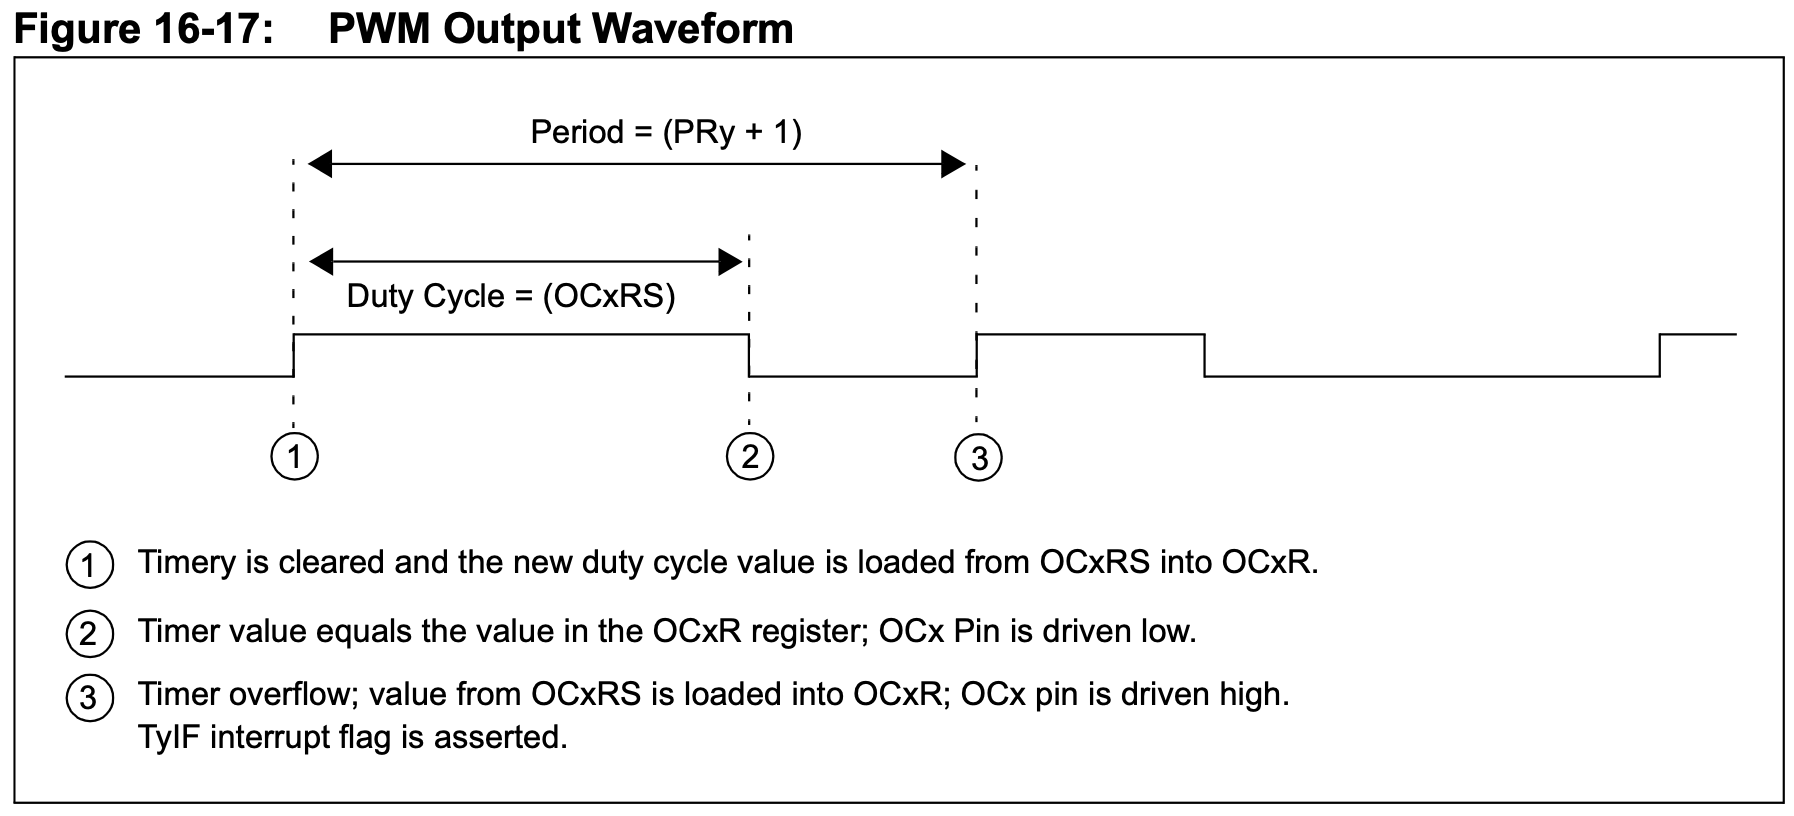
\includegraphics[width=0.8\linewidth]{PWM_output_waveform.png}
        \label{fig:PWM_output_waveform.png}
      \end{figure}

    \item \textbf{Calculations}
      \begin{equation*}
        \begin{aligned}
          T_{\text{PWM}}                      & = (PR + 1) \times T_{\text{PB}}  \times \text{Timer Prescale Value}                                \\
          2^{\text{PWMResolution}}            & = \frac{T_{\text{PWM}}}{T_{\text{timer}} }                                                         \\
          \text{PWMResolution} \text{ (bits)} & = \log_2 \left( \dfrac{F_{\text{PB}} }{F_{\text{PWM}} \times \text{Timer Prescale Value}}  \right) \\
        \end{aligned}
      \end{equation*}

    \item \textbf{Configuration}
      \begin{enumerate}[label = \arabic*.]
        \item Set the PWM period by writing to the selected timer period register (\verb|PRy|).
        \item Set the PWM duty cycle by writing to the \verb|OCxRS| register.
        \item \cprotect\textbf{Write the \verb|OCxR| register with the initial duty cycle.}
        \item Enable interrupts, if required, for the timer and Output Compare modules. The output compare interrupt is required for PWM Fault pin utilization.
        \item Configure the Output Compare module for one of two PWM Operation modes by writing to the Output Compare mode bits, \verb|OCM<2:0>| (\verb|OCxCON<2:0>|).
        \item Set the \verb|TMRy| prescale value and enable the time base by setting \verb|TON| (\verb|TxCON<15>|)\verb| = 1|.
      \end{enumerate}
  \end{enumerate}

\section*{L10 --- Analog-to-Digital Conversion (ADC)}
  \begin{enumerate}[label = \arabic*.]
    \item \textbf{Nyquist Theorem}
      \par A bandlimited analog signal that has been sampled can be perfectly reconstructed from an infinite sequence of samples if the sampling rate \( f_s \) exceeds \( 2 f_{max} \) samples per second, where \( f_{max} \) is the highest frequency in the original signal. % chktex 35
      \par \textbf{In short:}
      \begin{equation*}
        f_{\text{sampling}} > 2 f_{\text{original}}
      \end{equation*}

    \item \textbf{Aliasing}
      \par Aliasing is when the digital signal appears to have a different frequency than the original analog signal.
      \par If the analog signal does contain frequency components larger than \( f_s/2 \), then there will be an aliasing error.
      \par Aliasing example:
      \begin{figure}[H]
        \centering
        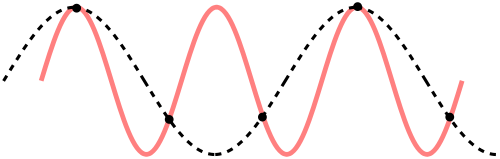
\includegraphics[width=0.4\linewidth]{Nyquist_aliasing_example.png}
        \caption{The samples of two sine waves can be identical when at least one of them is at a frequency above half the sample rate.}
        \label{fig:Nyquist_aliasing_example.png}
      \end{figure}

    \item \textbf{Steps to convert analog signal to digital signal}
      \begin{enumerate}[label = \arabic*.]
        \item \textbf{Sampling \& Holding}
          \begin{figure}[H]
            \centering
            \begin{subfigure}[b]{0.45\linewidth}
              \centering
              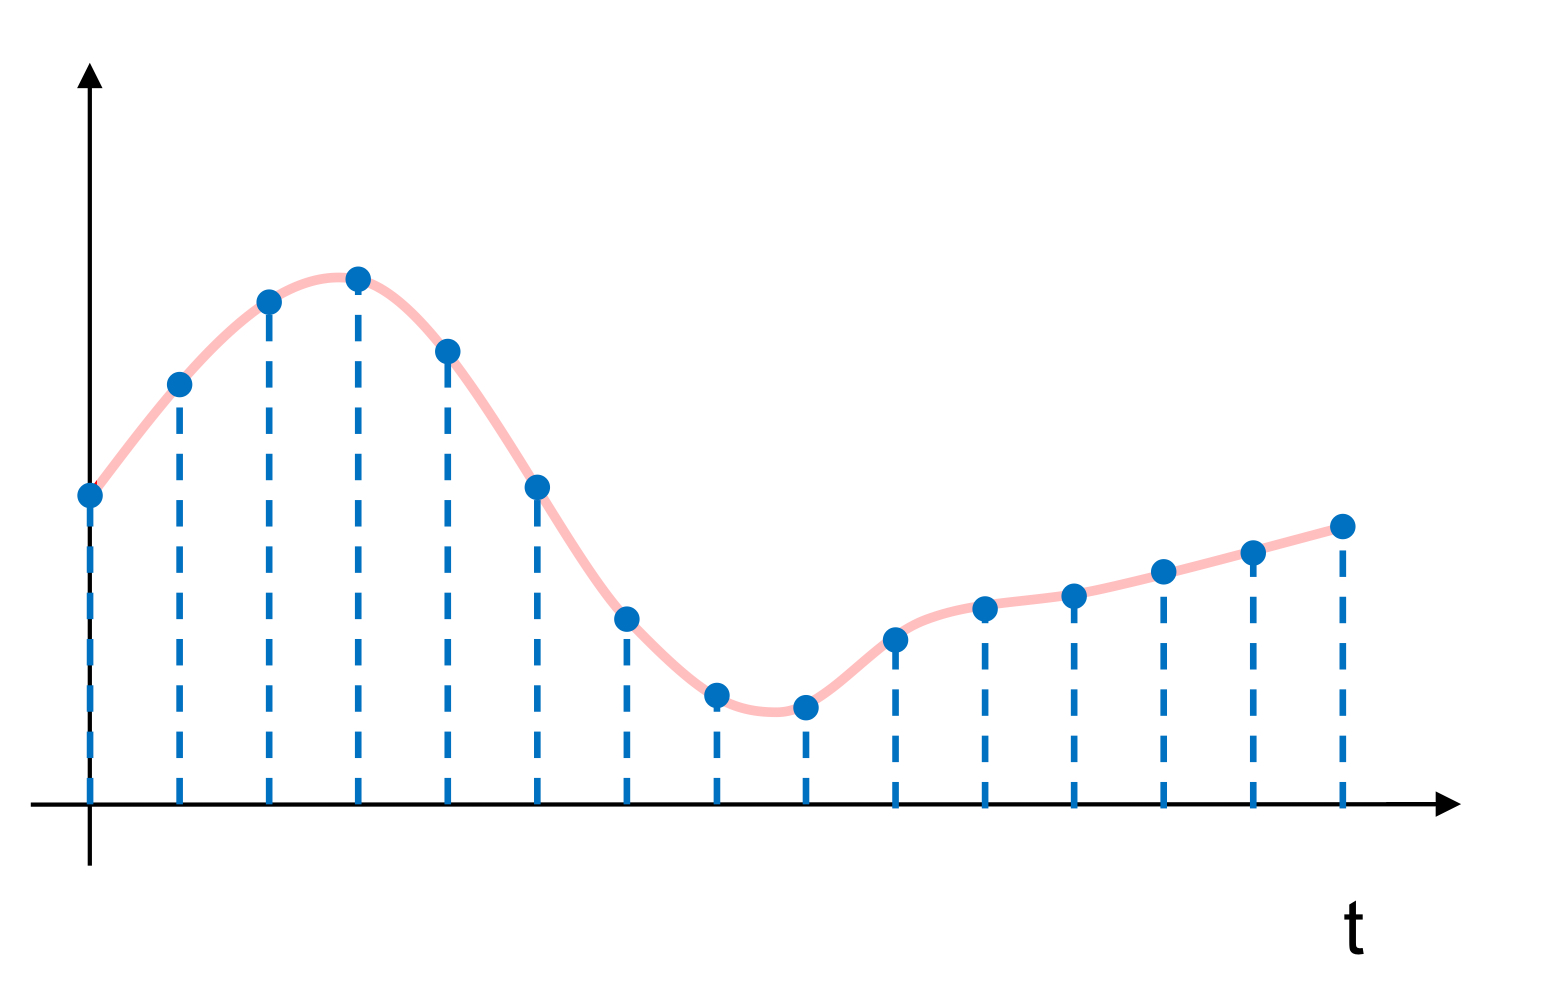
\includegraphics[width=0.9\linewidth]{ADC_sampling.jpeg}
              \caption{Sampling}
              \label{subfig:ADC_sampling.jpeg}
            \end{subfigure}
            \begin{subfigure}[b]{0.45\linewidth}
              \centering
              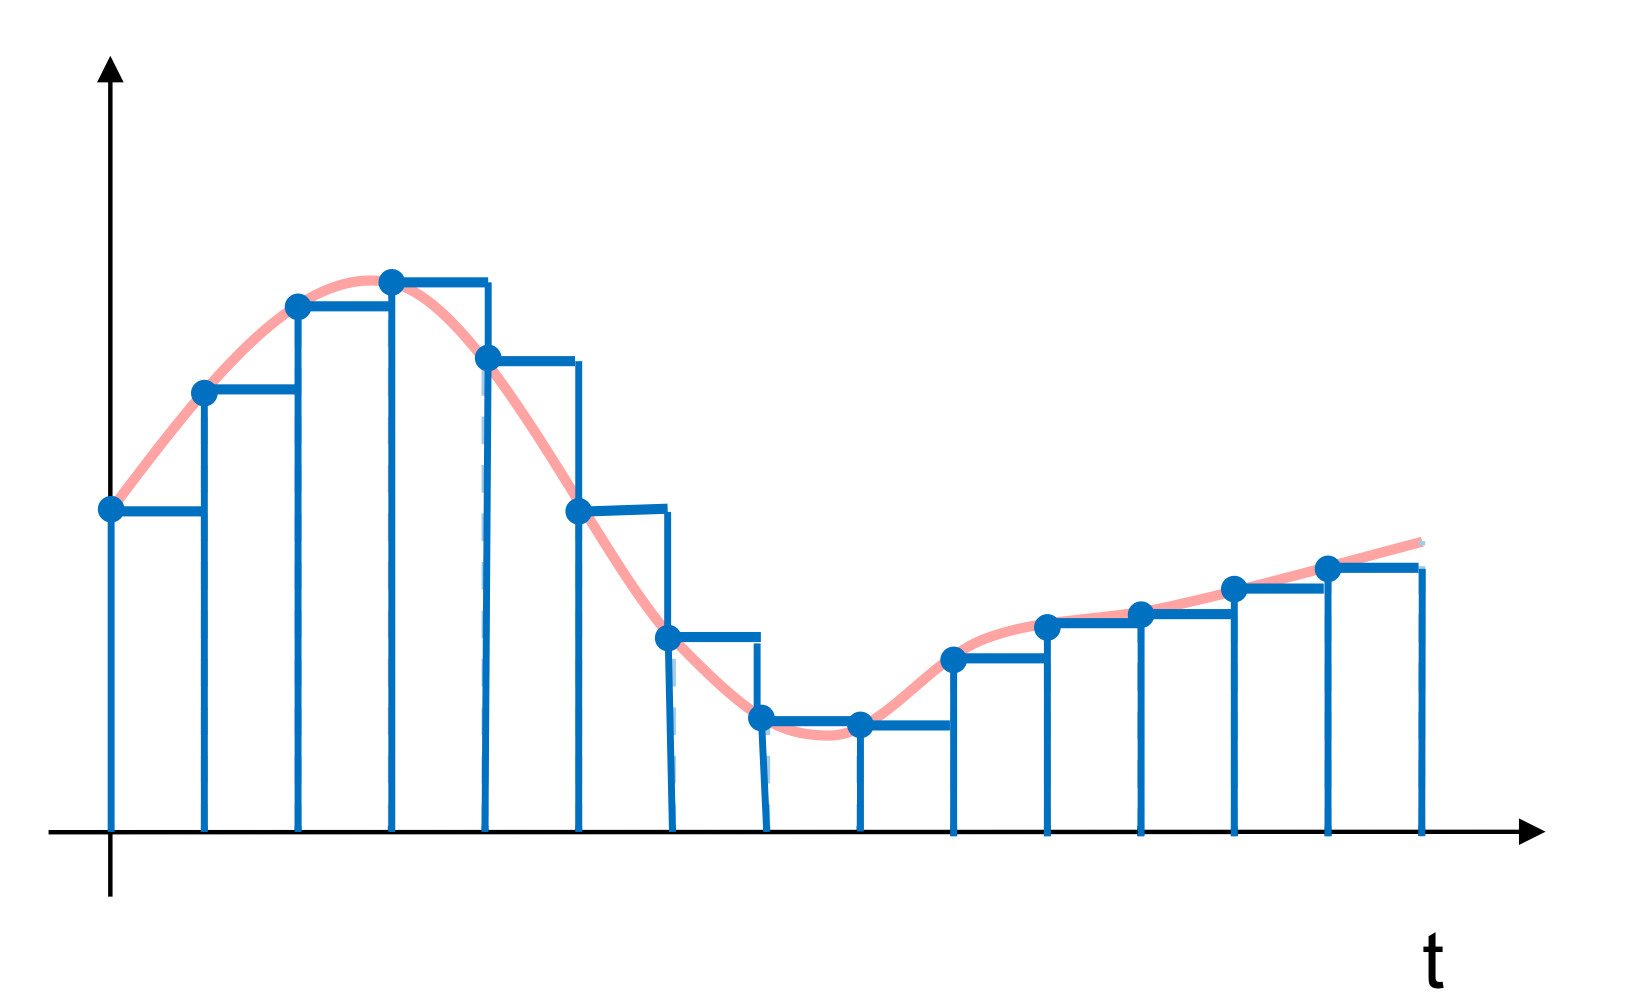
\includegraphics[width=0.9\linewidth]{ADC_holding.jpeg}
              \caption{Holding}
              \label{subfig:ADC_holding.jpeg}
            \end{subfigure}
            \label{fig:sampling_and_holding}
          \end{figure}

        \item \textbf{Quantization}
          \begin{itemize}[leftmargin = 1cm]
            \item Separating the input signal into a discrete states with \( K \) increments
            \item \( K = 2^N \)
            \item \( N \) is the number of bits of the ADC
          \end{itemize}

        \item \textbf{Coding}
          \par Assigning a unique digital code to each state for input into the microprocessor

          \begin{figure}[H]
            \centering
            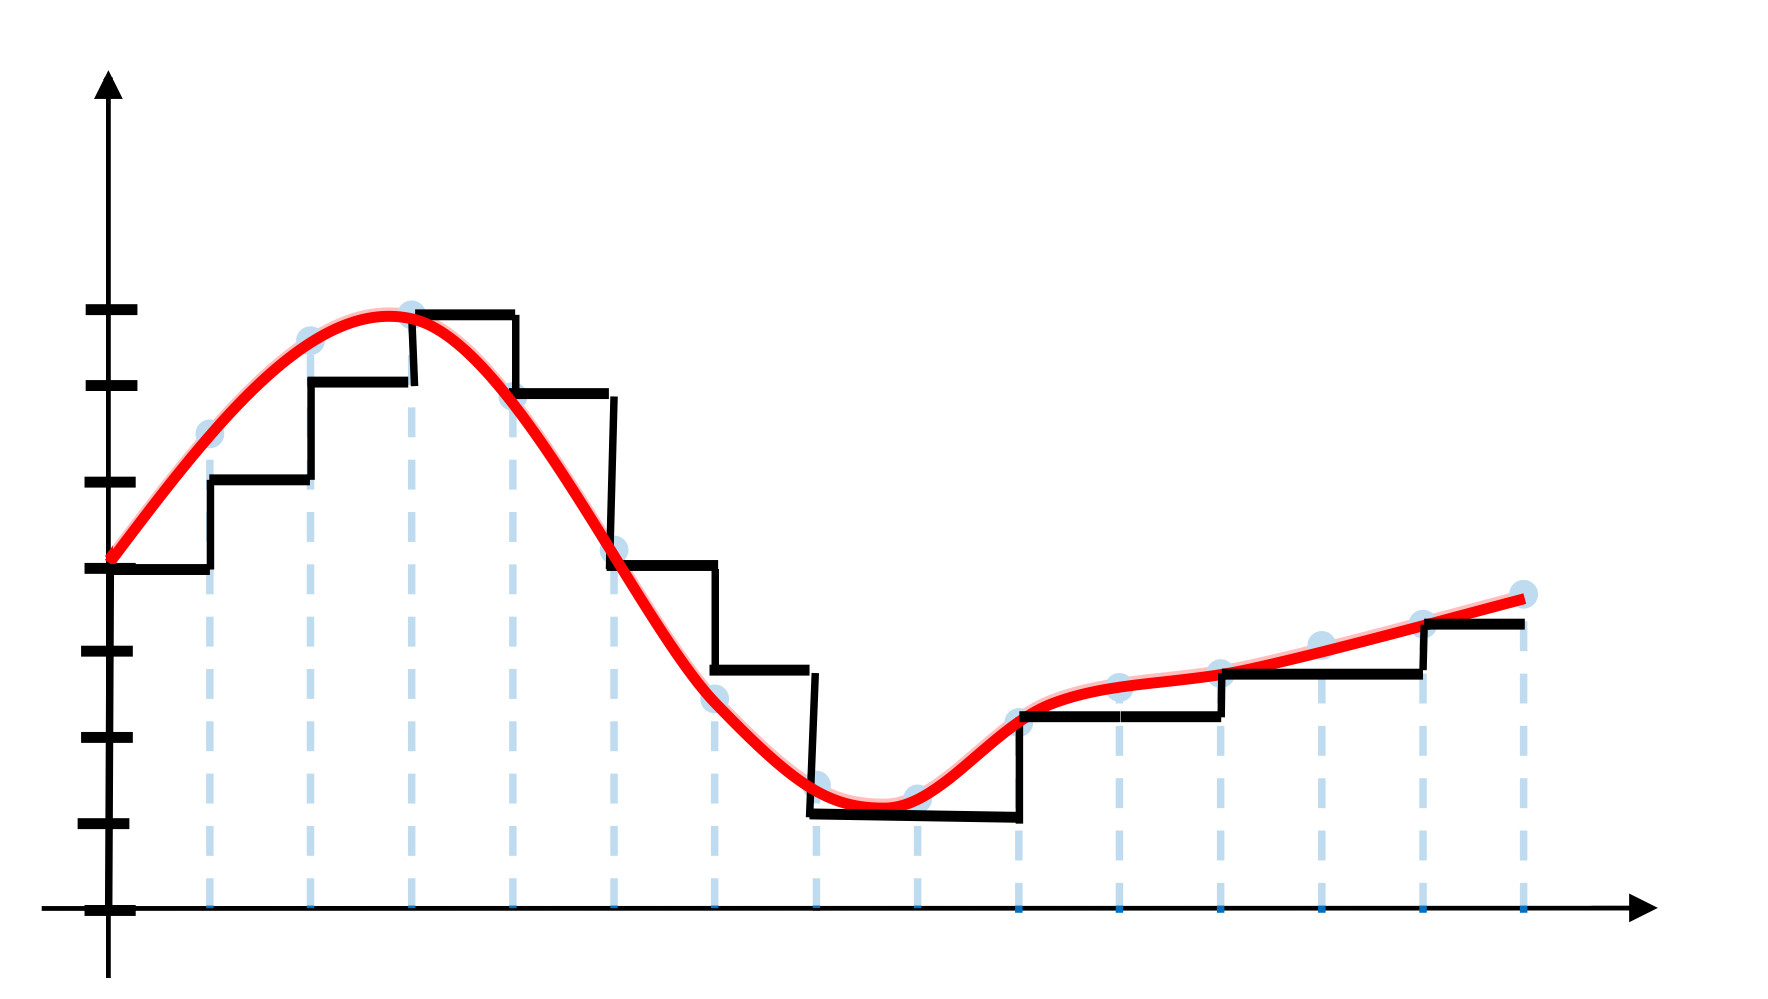
\includegraphics[width=0.5\linewidth]{ADC_quantization_and_encoding.jpeg}
            \caption{Quantization and Coding}
            \label{fig:ADC_quantization_and_encoding.jpeg}
          \end{figure}

      \end{enumerate}

    \item \textbf{Resolution}
      \par Amount of information the digital code is able to represent
      \begin{equation*}
        Q = \frac{V_{\text{max}} - V_{\text{min}} }{2^N}
      \end{equation*}
      \par \textbf{Larger range means lower resolution given fixed number of bits}

    \item \textbf{Quantization error}
      \par How far off discrete value is from actual value
      \begin{equation*}
        \text{Quantization error} = \frac{1}{2} Q
      \end{equation*}
      \par \textbf{Larger range means larger quantization error}

    \item \textbf{Digital representation}
      \begin{figure}[H]
        \centering
        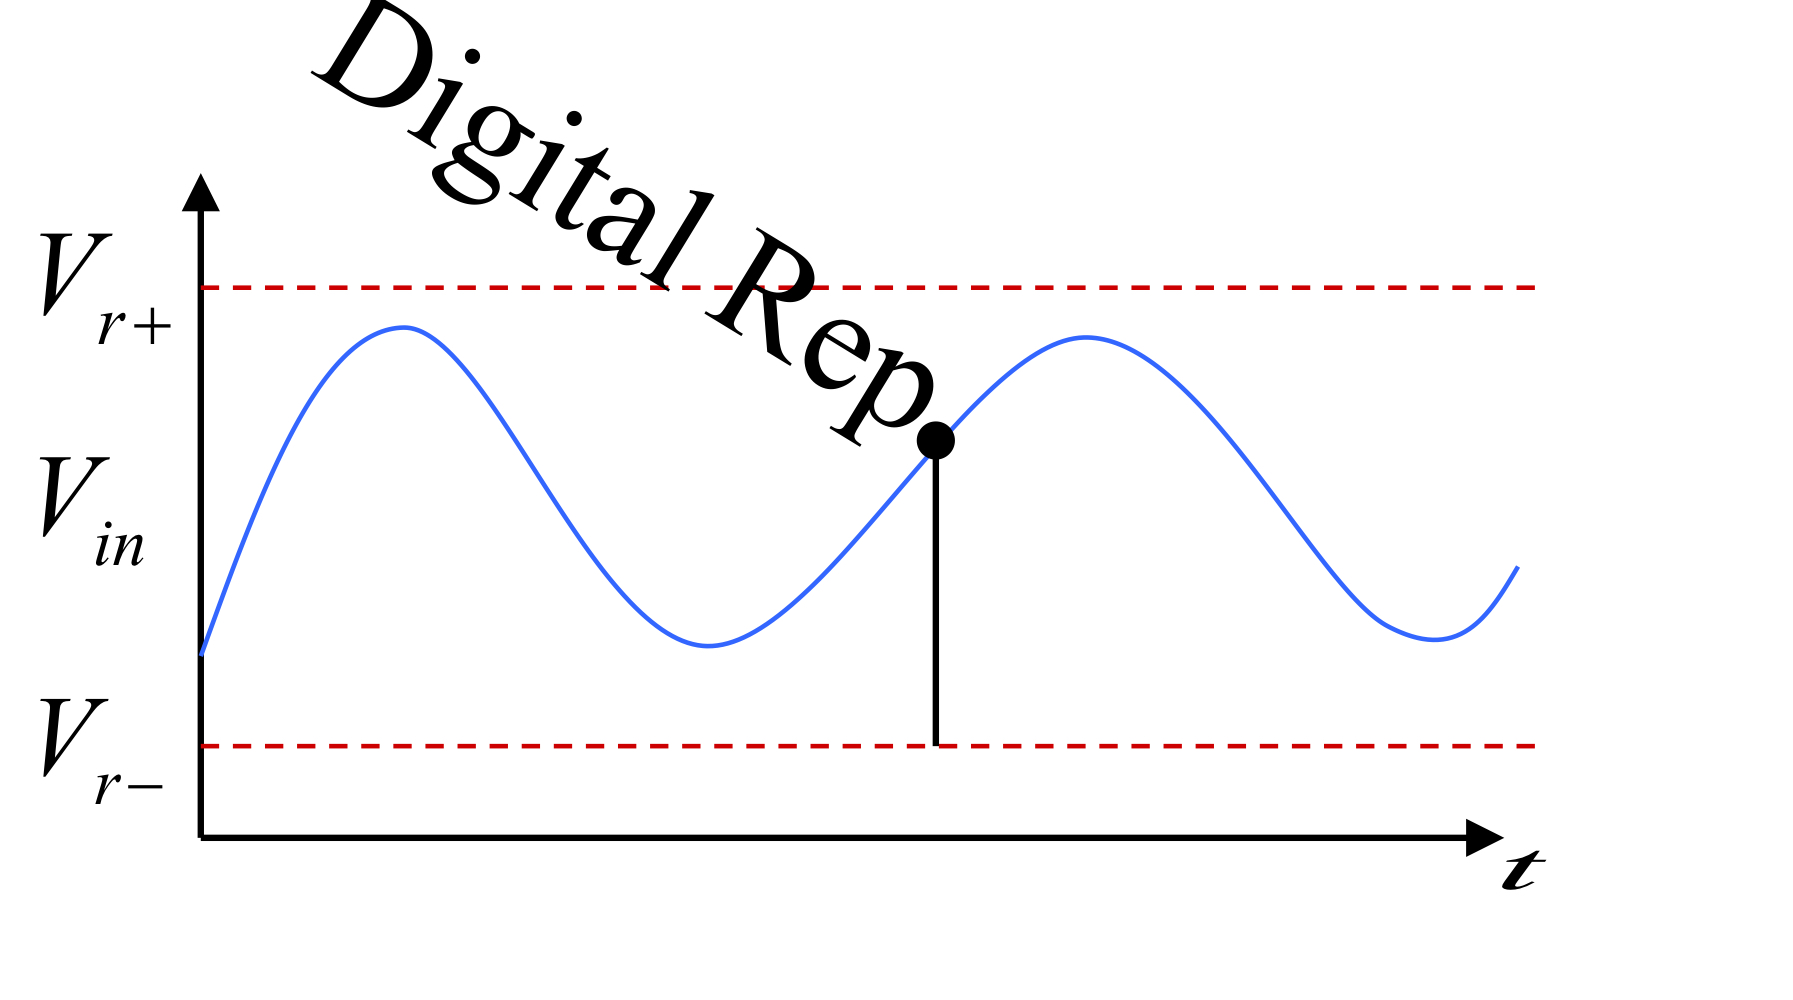
\includegraphics[width=0.4\linewidth]{ADC_digital_representation.jpeg}
        \label{fig:ADC_digital_representation.jpeg}
      \end{figure}

      \begin{equation*}
        \begin{aligned}
          \text{Digital Rep} & = 2^N \cdot \frac{V_{in} - V_{r-} }{V_{r+} - V_{r-} }            \\
          V_{in}             & = \text{Digital Rep} \cdot \frac{V_{r+} - V_{r-} }{2^N} + V_{r-} \\
        \end{aligned}
      \end{equation*}

    \item \textbf{ADC implementation}
      \begin{enumerate}[label = \arabic*.]
        \item \textbf{Method 1: Voltage Divider}
          \begin{figure}[H]
            \centering
            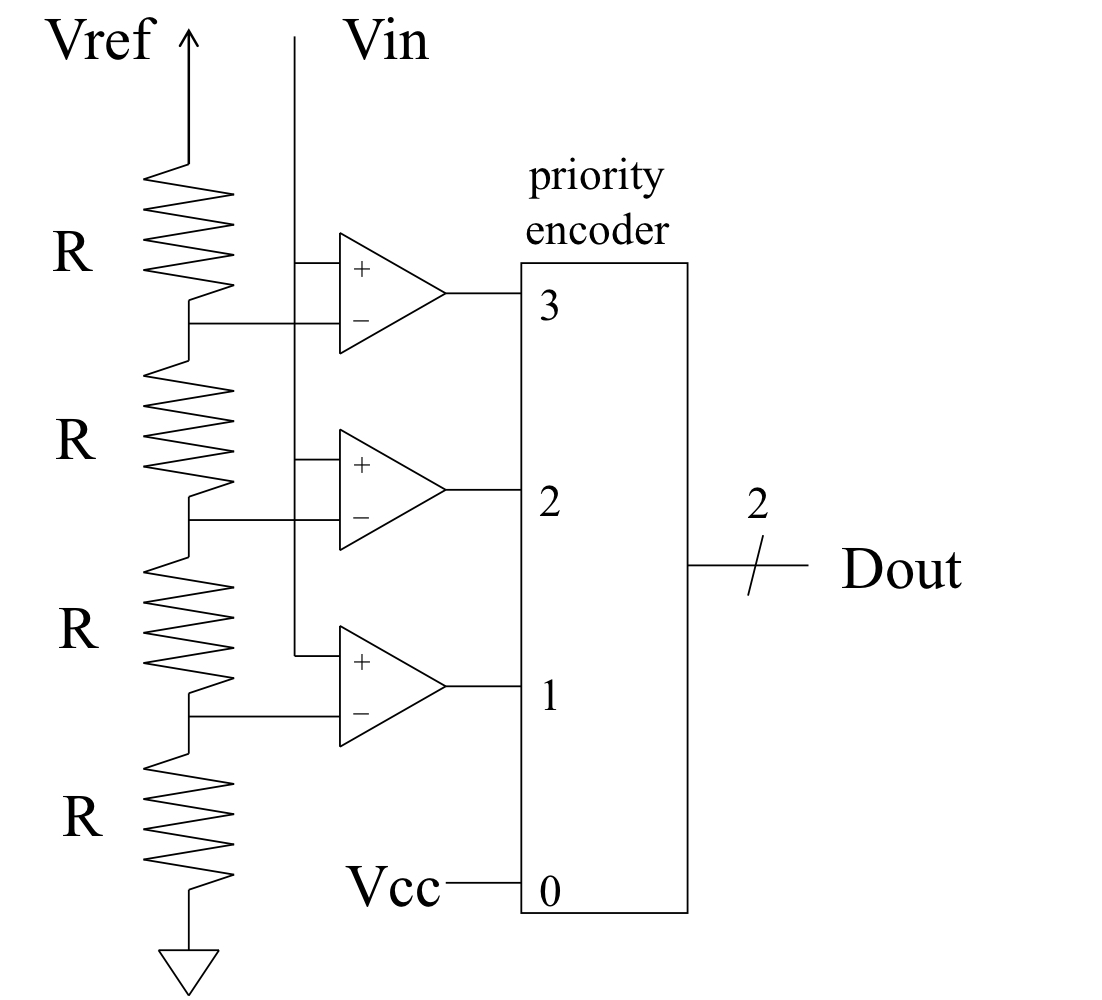
\includegraphics[width=0.4\linewidth]{Voltage_divider.jpeg}
            \caption{Voltage Divider}
            \label{fig:Voltage_divider.jpeg}
          \end{figure}

        \item \textbf{Method 2: Successive Approximation}
          \par Most used in PIC MCUs.
          \par Example: 4-bit resolution, \( 2^4 \) = 16 discrete representations
          \begin{itemize}[leftmargin = 1cm]
            \item B3 = 1 (upper half of 1/2)
            \item B2 = 0 (lower half of 3/4)
            \item B1 = 0 (lower half of 5/8)
            \item B0 = 1 (upper half of 9/16)
          \end{itemize}
          \begin{figure}[H]
            \centering
            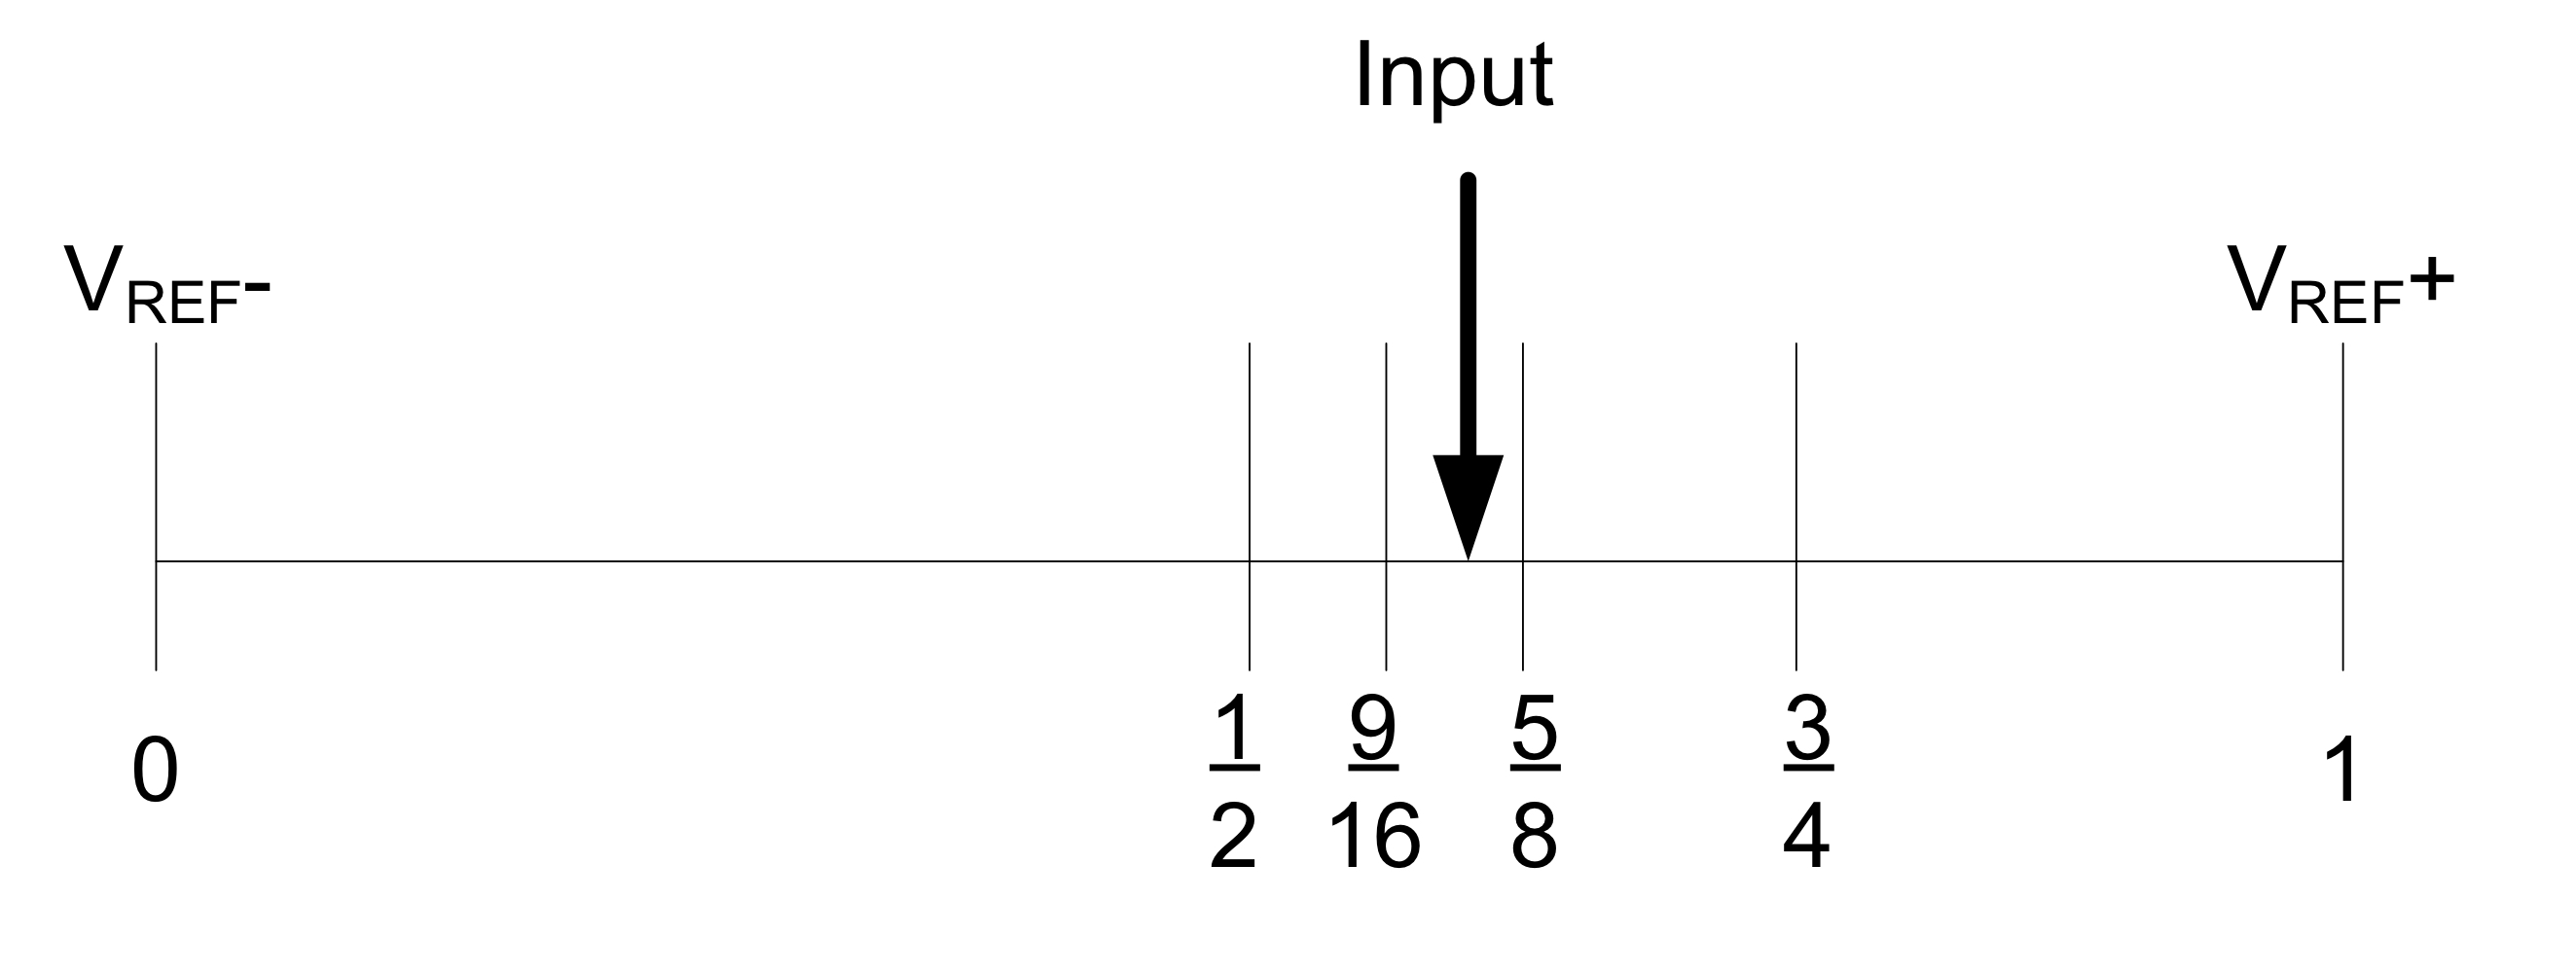
\includegraphics[width=0.6\linewidth]{Successive_approximation.jpeg}
            \caption{Successive Approximation}
            \label{fig:Successive_approximation.jpeg}
          \end{figure}

      \end{enumerate}

    \item \textbf{ADC of PIC32}
      \begin{itemize}[leftmargin = 1cm]
        \item 10 bits, i.e. \( N = 10 \).
        \item 16 analog input channels
        \item 8 conversion result formats
        \item Up to 16 words storage for converted digital value
        \item Selectable conversion trigger source
      \end{itemize}


    \item \textbf{ADC Block Diagram}
      \begin{figure}[H]
        \centering
        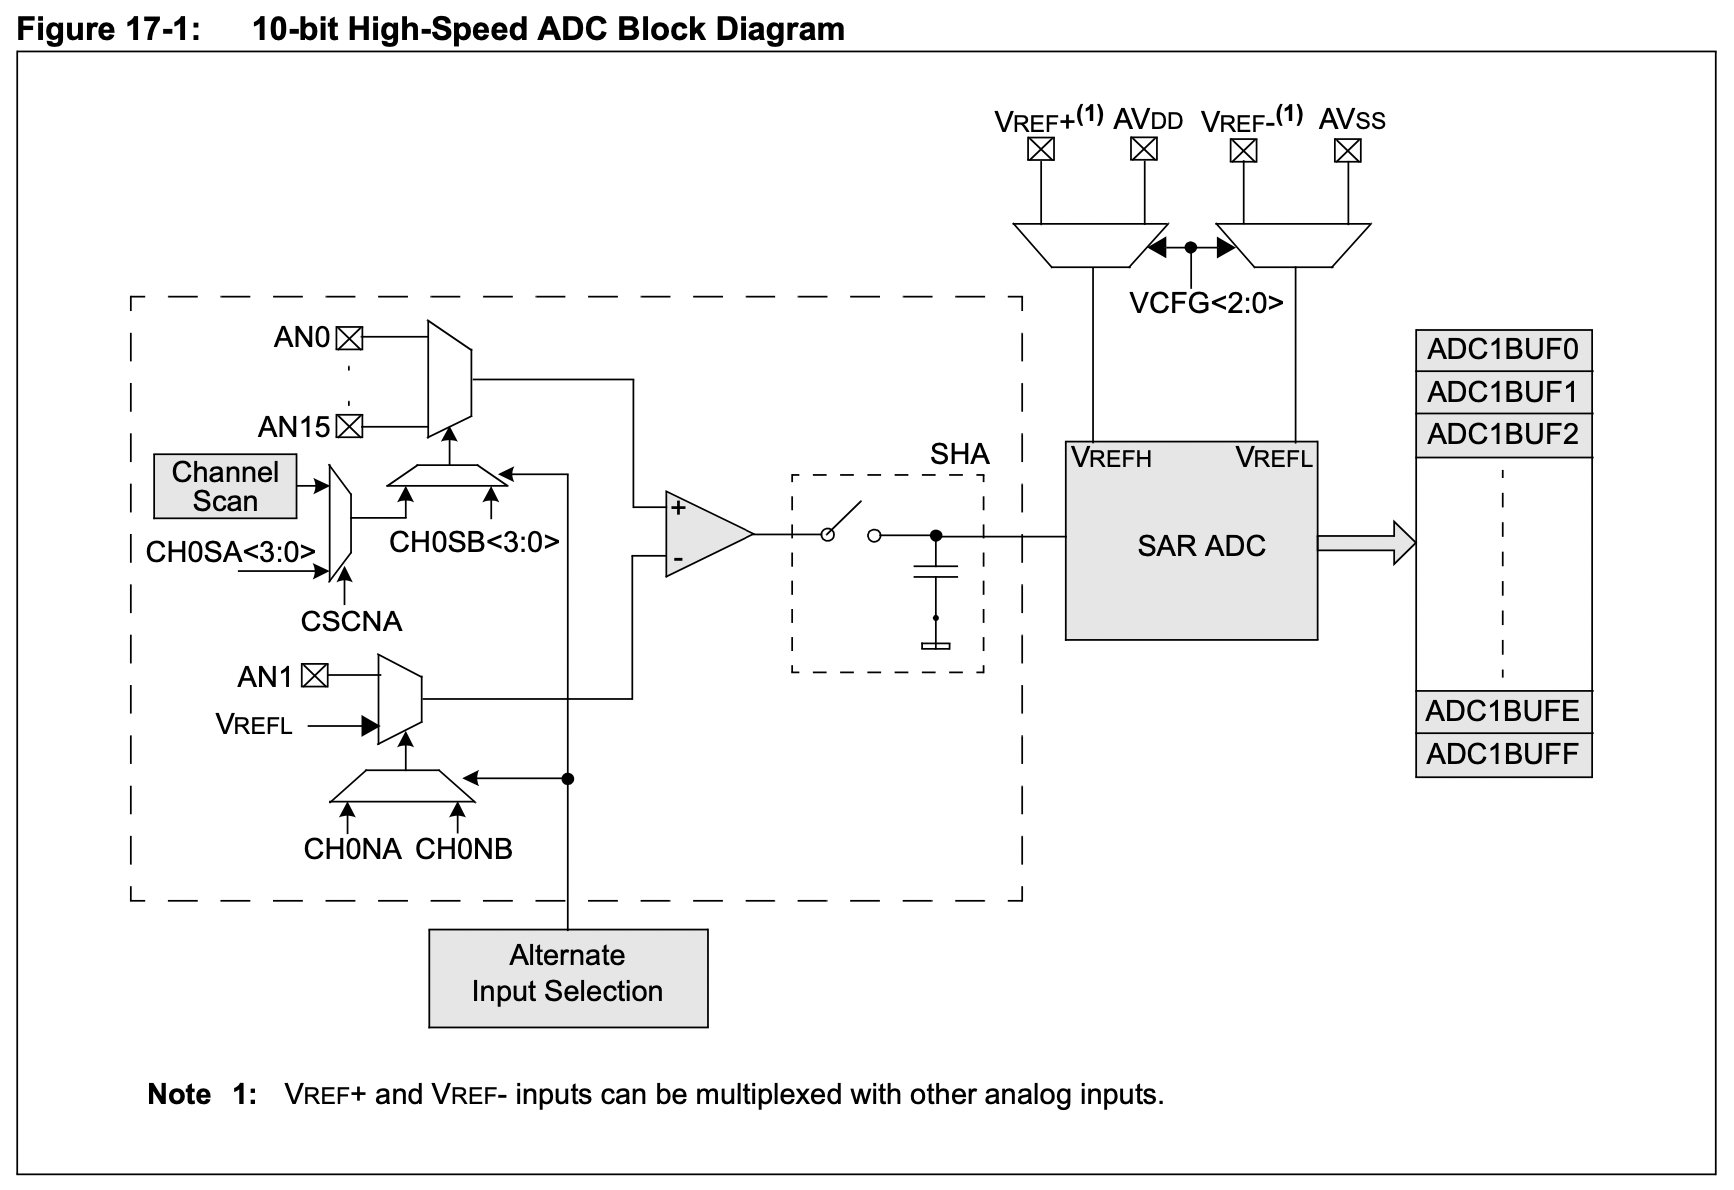
\includegraphics[width=0.9\linewidth]{ADC_block_diagram.png}
        \label{fig:ADC_block_diagram.png}
      \end{figure}

    \item \textbf{ADC time taken}
      \begin{enumerate}[label = \arabic*.]
        \item \textbf{Acquisition}
          \par Analog signal sampled and hold
          \par SHA\@: Sample and Hold Amplifier
          \par Enough time must be given, variable
          \par Set by \verb|SAMC| (\verb|AD1CON3<12:8>|)
        \item \textbf{Conversion}
          \par Sampled analog signal converted to digital
          \par Requires \( 12 T_{AD}  \) time to finish
          \begin{itemize}[leftmargin = 1cm]
            \item One \( T_{AD}  \) per bit + 2 additional \( T_{AD} \)
            \item \( T_{AD} \) is configurable, \( > 65 \) ns
          \end{itemize}
          \( T_{AD} \) source can be selected from internal RC source or prescaled \verb|PBCLK| by configuring \verb|ADRC| (\verb|AD1CON3<15>|)
      \end{enumerate}

      \begin{figure}[H]
        \centering
        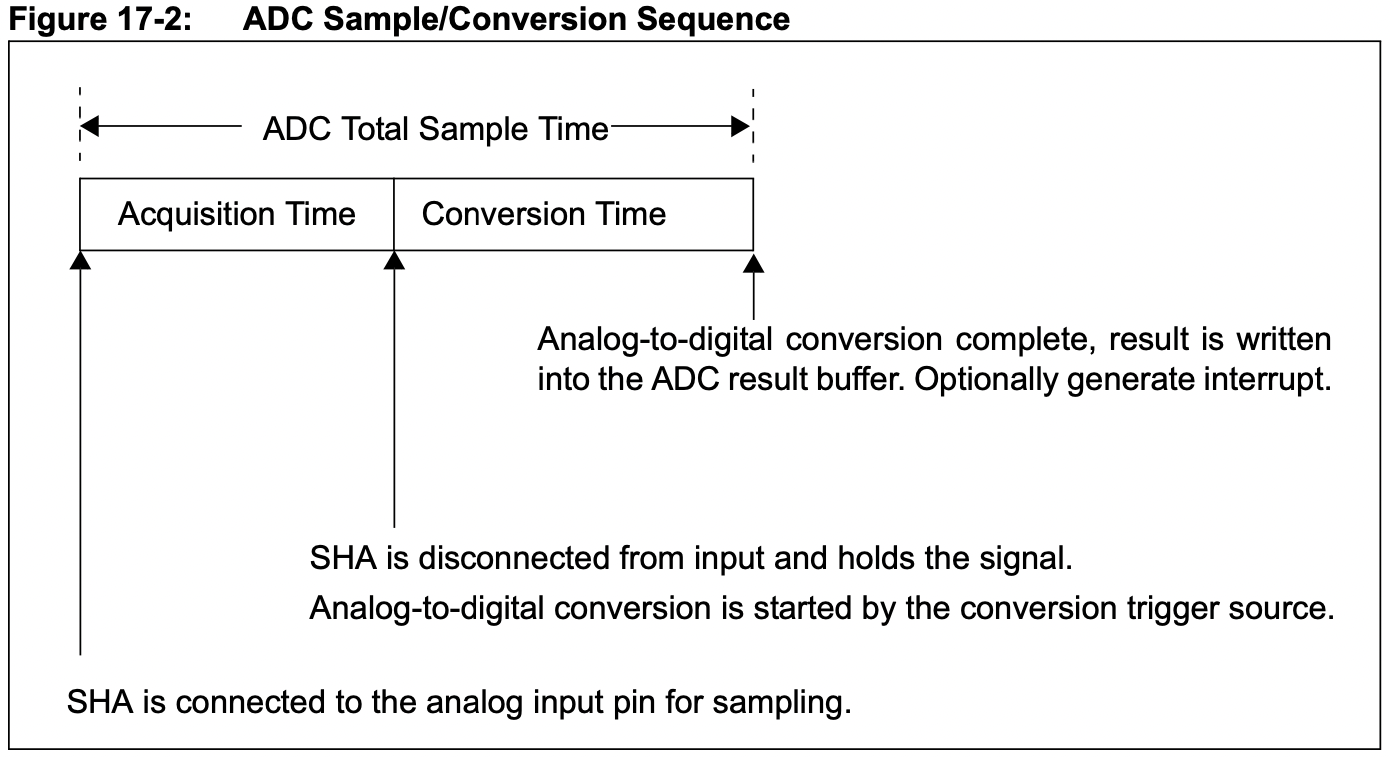
\includegraphics[width=0.8\linewidth]{ADC_sequence.png}
        \label{fig:ADC_sequence.png}
      \end{figure}

      \begin{figure}[H]
        \centering
        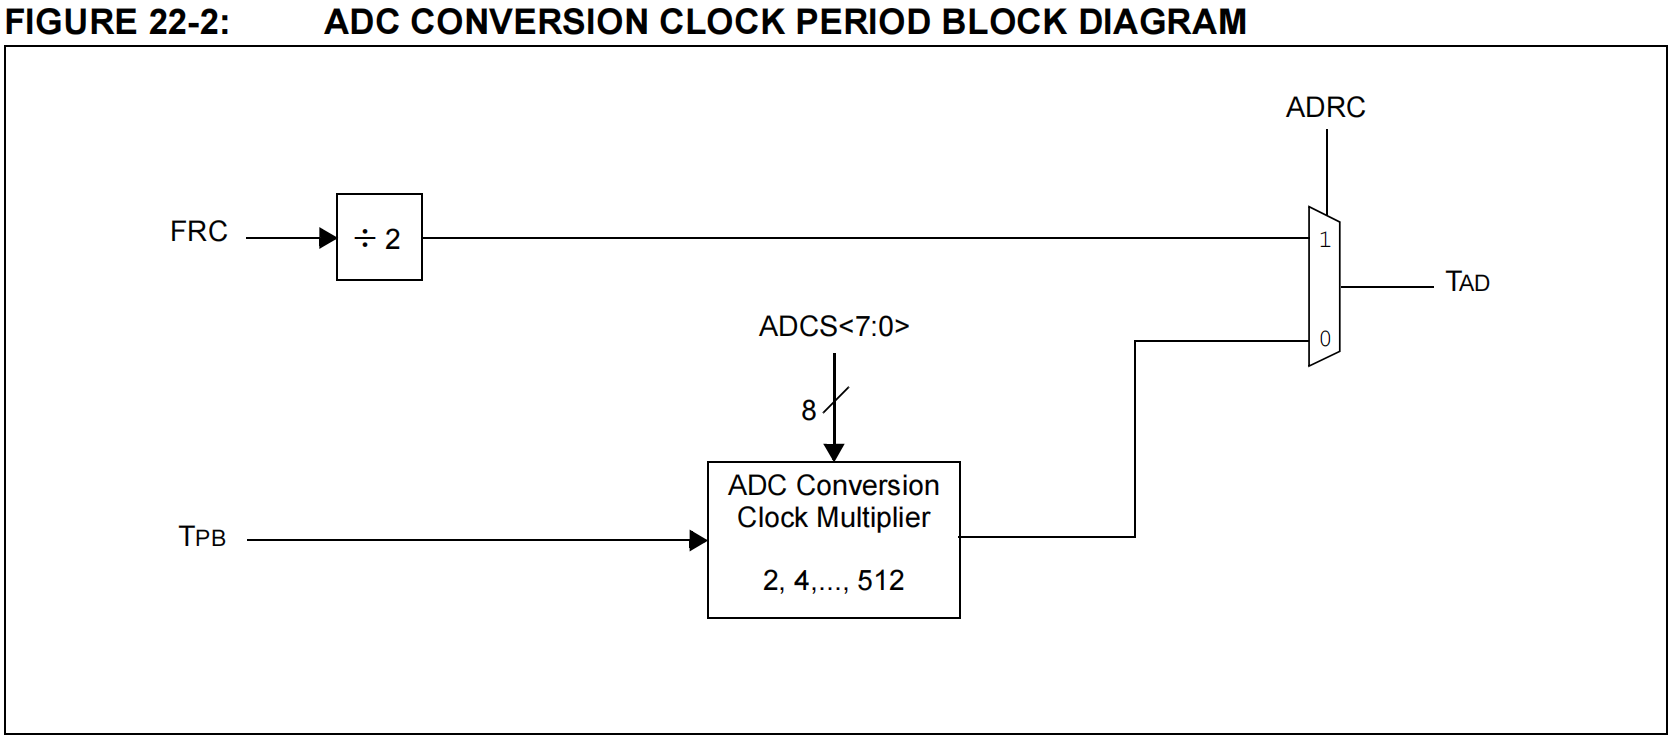
\includegraphics[width=0.8\linewidth]{ADC_clock_source.png}
        \label{fig:ADC_clock_source.png}
      \end{figure}

    \item \textbf{ADC Modes}
      \begin{itemize}[leftmargin = 1cm]
        \item Manual
          \begin{itemize}[leftmargin = 1cm]
            \item Manually start acquisition
            \item Manually start conversion
          \end{itemize}
        \item Automatic
          \begin{itemize}[leftmargin = 1cm]
            \item Continuous conversion sequence
            \item Multiple sample and conversions
          \end{itemize}
        \item Scan mode
          \begin{itemize}[leftmargin = 1cm]
            \item Scan through multiple inputs
            \item Inputs selectable
            \item MUX A only
          \end{itemize}
        \item Alternate scan mode
          \begin{itemize}[leftmargin = 1cm]
            \item MUX A and MUX B
            \item Input selectable
          \end{itemize}
      \end{itemize}

      \begin{figure}[H]
        \centering
        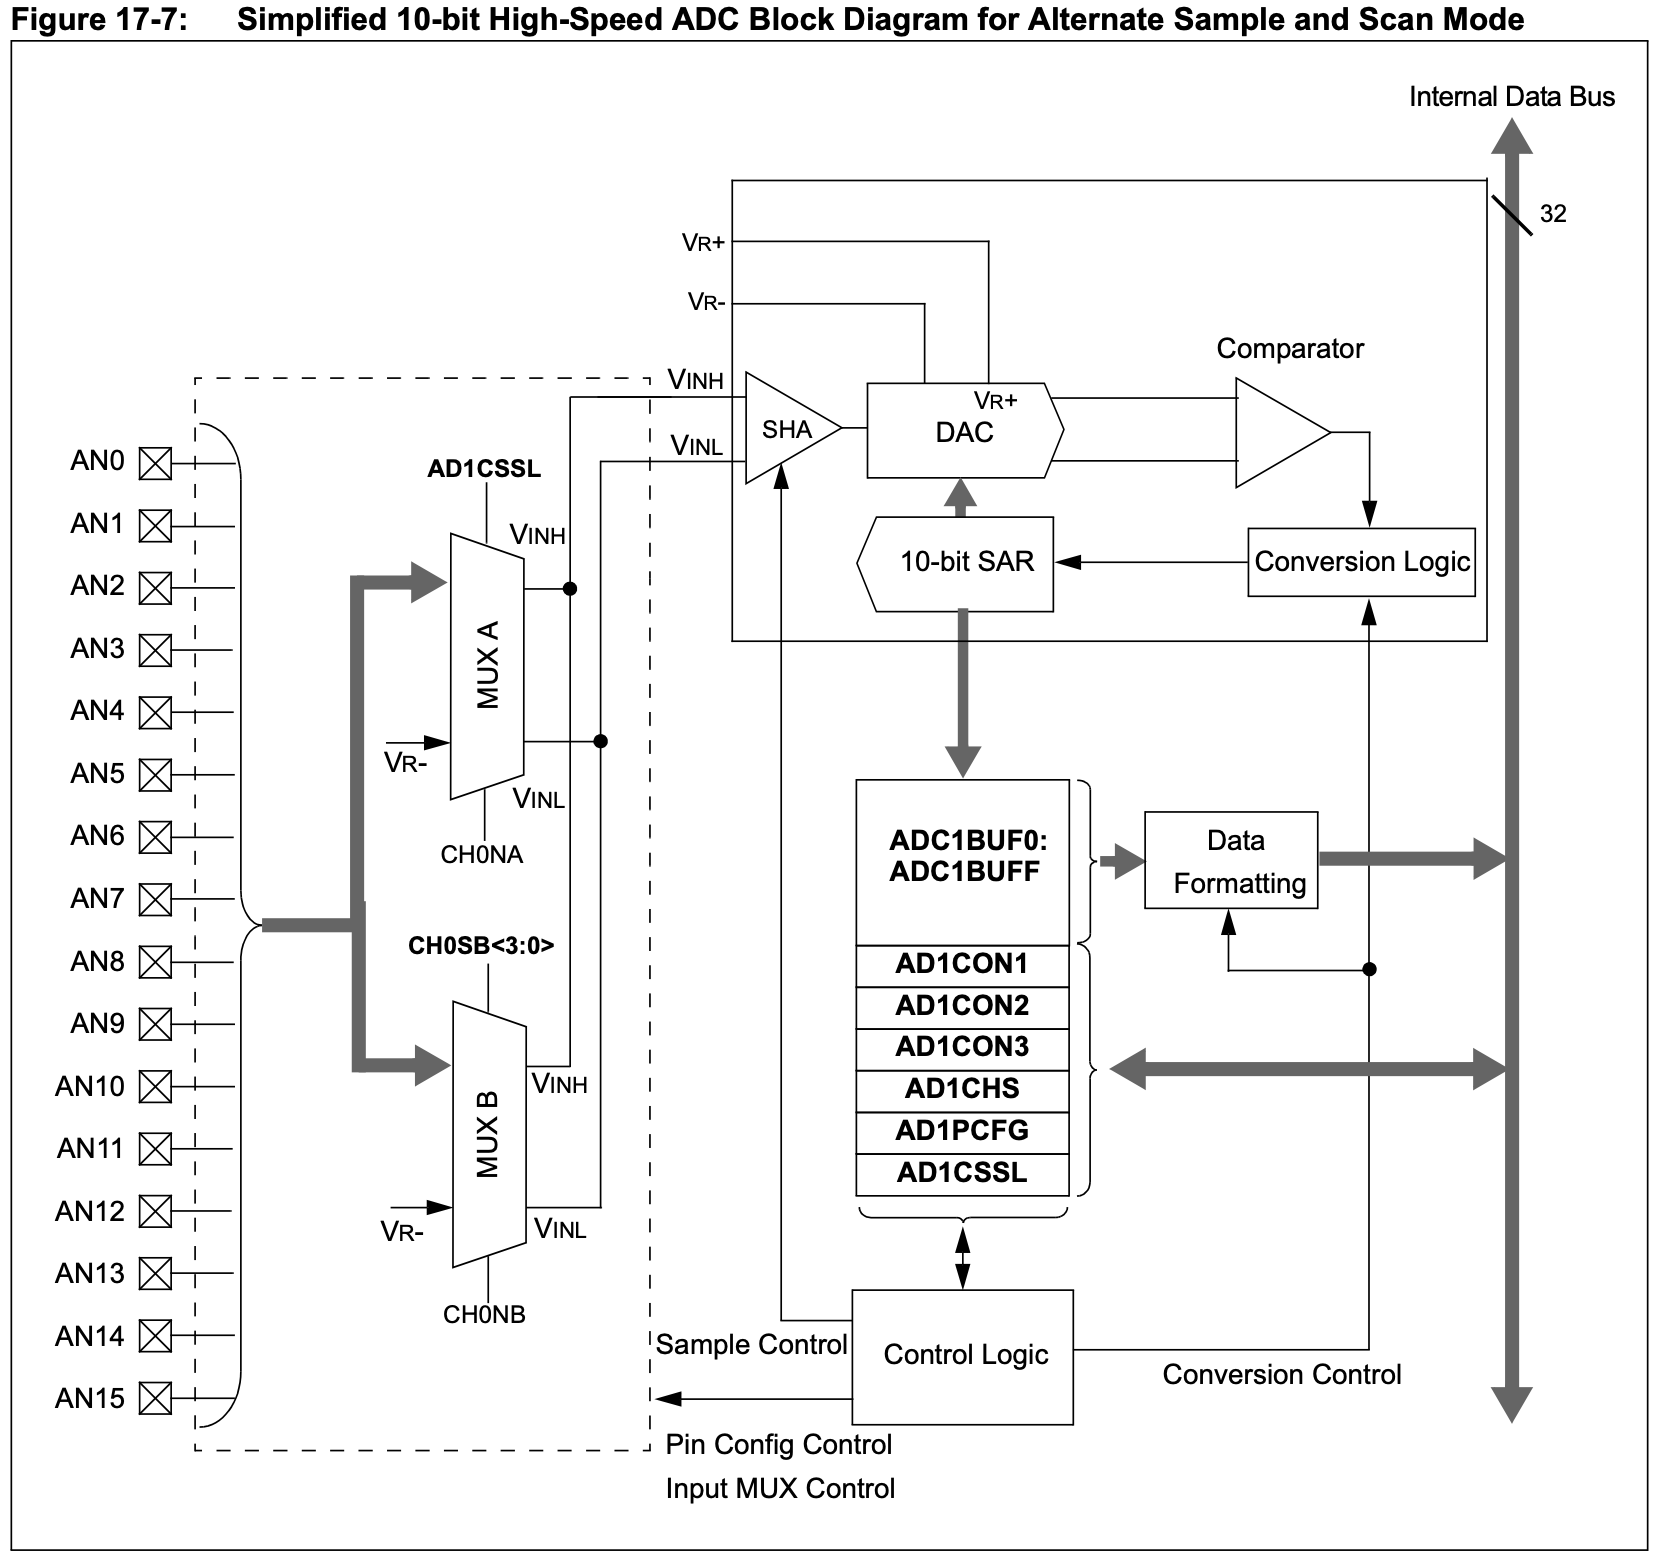
\includegraphics[width=0.6\linewidth]{ADC_channal_selection.png}
        \label{fig:ADC_channal_selection.png}
      \end{figure}

    \item \textbf{ADC Interrupt}
      \par Configured by \verb|SMPI<2:0>| (\verb|AD1CON2<5:2>|). Can generate interrupt after 1 -- 16 samples.
      \par The next sequence starts filling the buffer from the top even if the number of samples in the previous sequence was less than 16.

    \item \textbf{ADC Setup}
      \begin{enumerate}[label = \arabic*.]
        \item Configure the analog port pins in \verb|AD1PCFG<15:0>|.
        \item Select the analog inputs to the ADC multiplexers in \verb|AD1CHS<32:0>|.
        \item Select the format of the ADC result using \verb|FORM<2:0>| (\verb|AD1CON1<10:8>|).
        \item Select the sample clock source using \verb|SSRC<2:0>| (\verb|AD1CON1<7:5>|).
        \item Select the voltage reference source using \verb|VCFG<2:0>| (\verb|AD1CON2<15:13>|).
        \item Select the Scan mode using \verb|CSCNA| (\verb|AD1CON2<10>|).
        \item Set the number of conversions per interrupt \verb|SMP<3:0>| (\verb|AD1CON2<5:2>|), if interrupts are to be used.
        \item Set Buffer Fill mode using \verb|BUFM| (\verb|AD1CON2<1>|).
        \item Select the MUX to be connected to the ADC in \verb|ALTS| \verb|AD1CON2<0>|.
        \item Select the ADC clock source using \verb|ADRC| (\verb|AD1CON3<15>|).
        \item Select the sample time using \verb|SAMC<4:0>| (\verb|AD1CON3<12:8>|), if auto-convert is to be used.
        \item Select the ADC clock prescaler using \verb|ADCS<7:0>| (\verb|AD1CON3<7:0>|).
        \item Turn the ADC module on using \verb|AD1CON1<15>|.
        \item To configure ADC interrupt (if required):
          \begin{enumerate}[label = \alph*)] % chktex 9 chktex 10
            \item Clear the \verb|AD1IF| bit (\verb|IFS1<1>|).
            \item Select ADC interrupt priority \verb|AD1IP<2:0>| (\verb|IPC<28:26>|) and subpriority \verb|AD1IS<1:0>| (\verb|IPC<24:24>|) if interrupts are to be used.
          \end{enumerate}
        \item Start the conversion sequence by initiating sampling.
          \begin{itemize}[leftmargin = 1cm]
            \item \textit{Manual mode}: setting \verb|1| to \verb|SAMP| bit (\verb|AD1CON1<1>|).
              \par Software must manually manage the start and end of the acquisition period by setting and then clearing the SAMP bit after the desired acquisition period has elapsed.
            \item \textit{Auto-sample mode}: settings \verb|1| to \verb|ASAM| bit (\verb|AD1CON1<2>|)
              \par Acquisition is automatically started after a conversion is completed. Auto-Sample mode can be used with any trigger source other than manual.
          \end{itemize}
      \end{enumerate}
      \par \textbf{Note:} Steps 1 through 12, above, can be performed in any order, but Step 13 must be the final step in every case.

    \item \textbf{DONE bit}

      \par The \verb|DONE| bit (\verb|AD1CON1<0>|) is set when a conversion sequence is complete.
      \begin{itemize}[leftmargin = 1cm]
        \item In Manual mode:
          \par The \verb|DONE| bit is persistent.
          \par Remains set until it is cleared by software.
          \par Can be polled to determine when the conversion has completed.
        \item In all automatic sample modes (\verb|ASAM| bit = 1):
          \par the DONE bit is not persistent.
          \par Set at the end of a conversion sequence and cleared by hardware when the next acquisition is started.
          \par Polling the DONE bit is not recommended when operating the ADC in automatic modes.
          \par The \verb|AD1IF| flag bit (\verb|IFS1<1>|) is latched after a conversion sequence is completed and can therefore be polled.
      \end{itemize}



  \end{enumerate}


\end{document}